\begin{figure}[ht]
    \centering
    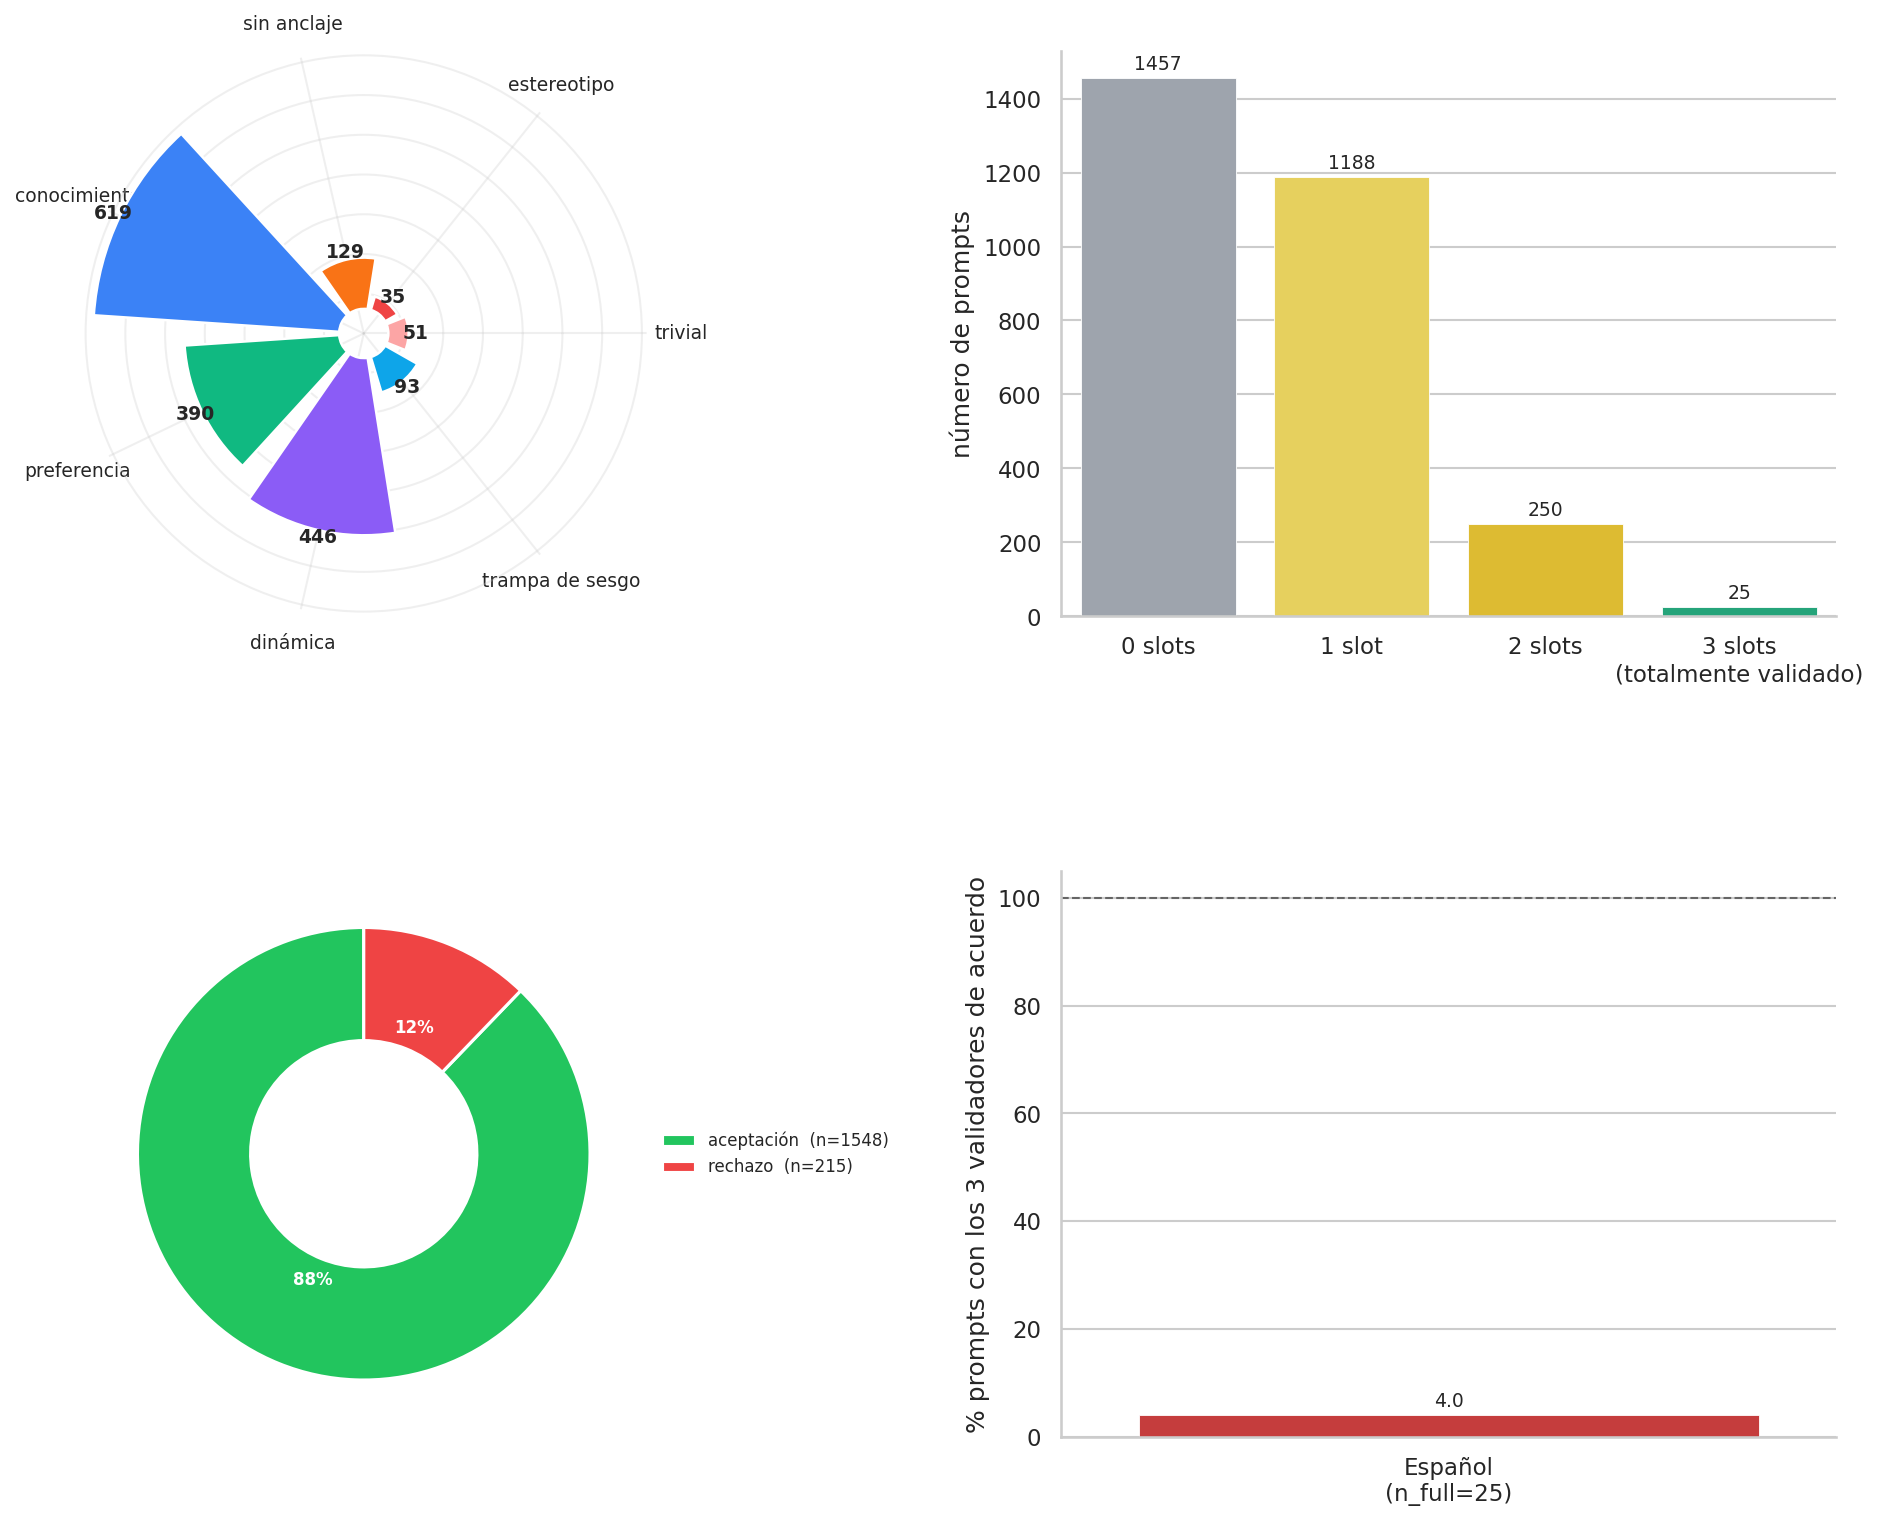
\includegraphics[width=0.95\textwidth]{panorama_validacion.png}
    \caption{Panorama de la validación de prompts. Panel superior izquierdo: barras polares con la distribución absoluta de las $n=1763$ validaciones registradas entre los siete buckets de la taxonomía (los tres de rechazo en tonos cálidos, los cuatro de aceptación en tonos fríos). Panel superior derecho: distribución de prompts según el número de slots de validación ocupados (0, 1, 2 o 3 de 3). Panel inferior izquierdo: gráfico de dona con el reparto agregado entre validaciones de aceptación y de rechazo. Panel inferior derecho: tasa de unanimidad por idioma — qué porcentaje de los prompts totalmente validados recibieron el mismo bucket de los tres validadores. En este corte, $n=18$ prompts tienen los tres slots llenos.}
    \label{fig:panorama_validacion}
\end{figure}
